%% ----------------------------------------------------------------------------
%% ----------------------------------------------------------------------------

\chapter{Experiments and Results}
This chapter describes the choice of various parameters for example in-sample length, $w_{i1}$ and shows the results obtained at different steps of our model implementation. The whole model was implemented using \textit{Python 3}. Python was chosen due to the availability of various modules for statistical analysis and also, easy wrapper modules for interfacing with different databases. In order to validate the SABM model, \textit{S\&P 500} index data is used. The values of \textit{closing price} and \textit{P/E ratio} were used for the in-sample period from 1990-01-01 to 2016-12-31 while out-of-sample analysis was done for the time from 2017-01-01 onwards. In following sections, the implementation details and results for back-testing, calibration, and final analysis are shown.

\section{Back-testing}
As explained in section \ref{steps} of Chapter 2, the agents use historical data of window length ($w_{i1}$) and generate strategy performances ($r_k(t)$ and $v_k(t)$) using back-testing. In general, it is preferred to choose window length to be large enough to get statistically good results. In our implementation, the window length for back-test was chosen to be \textbf{10 years} or approximately \textbf{2610 days}. We shift the back-test window and generate performances at each shift. The size of the shift was chosen as \textbf{22 days} and \textbf{252 days}. Using this approach, we generated two sets of results for the period of 2000 to 2017: one for the shift of 22 days and other for 252 days.

After choosing the window length and size of shift, we select different set of parameters for both strategies and generate performance for all parameters sets. The strategy parameters used by fundamentalists are \textit{entry threshold} and \textit{exit threshold} and are selected from the following paramter space: 

\begin{tabular}{ l l } 
 \textit{entry threshold} & : \quad 0, 1, 2, 3, 4, .... 37, 38, 39, 40, 41, 42,..... 76, 77, 78, 79]\\ 
 \textit{exit threshold} & : \quad 0, 1, 2, 3, 4, .... 37, 38, 39, 40, 41, 42,..... 76, 77, 78, 79]\\ 
\end{tabular}

The strategy performances are computed for all valid combinations of \textit{entry threshold} and \textit{exit threshold} from the space. All combinations with \textit{entry threshold} less than \textit{exit threshold} 
are considered. \par

Similarly, the parameters used in case of chartists strategy are \textit{slow window length}, \textit{fast window length}, \textit{entry threshold}, \textit{exit threshold} and \textit{stop loss}. For chartists, the performances are computed for all valid combinations of parameters from the given below parameter space. All combinations, for which \textit{fast window length} are less than \textit{slow window length}, are considered. The parameter space for chartists is as follow:

\begin{tabular}{ l l } 
 \textit{fast window length} & : \quad 5, 10, 15, 20, 25, 40, 60, 90, 120, 160, 200, 250 \\

\textit{slow window length} & : \quad 10, 15, 20, 25, 40, 60, 90, 120, 160, 200, 250, 300, 400, 500, 750 \\

\textit{entry threshold} & : \quad 1.0, 1.05, 1.1, 1.15, 1.2, 1.25, 1.5, 1.75, 2.0, 2.5 \\

\textit{exit threshold} & : \quad 1.0, 0.95, 0.9, 0.85, 0.8, 0.75, 0.5, 0.25 \\

\textit{exit threshold} & : \quad 0, 0.025, 0.05, 0.075, 0.1, 0.15, 0.2, 0.3, 0.4, 0.5, 0.6, 0.7, 1.0, 2.0 \\
\end{tabular}
\newline

We can observe that the parameter space selected for both strategies is significantly large. This was done to fulfill the requirement of huge $N_f$ and $N_c$, stated in steps for model creating model. An example of performance computed for chartists and fundamentalists can be seen in the table \ref{cp_perf} on page ~\pageref{cp_perf} and \ref{fp_perf} on page ~\pageref{fp_perf} respectively. It can be observed that we obtain different values of annual return and volatility for a different set of strategy parameters in case of both fundamentalist and chartist strategies. 

\begin{table}[h!]
\begin{center}
\begin{tabular}{|c|ccccc|ccc|}
\hline
   set\_idx &   fast\_wl &   slow\_wl &   entry\_th &   exit\_th &   stop\_loss &   annual\_return &   volatility &   maximum\_drawdown \\
\hline
        1 &         5 &        10 &       1    &      0.25 &       0     &       0.147496  &    0.133579  &            0.23971 \\
        2 &         5 &        10 &       1    &      0.25 &       0.025 &      -0.0794673 &    0.106909  &            3.60955 \\
        3 &         5 &        10 &       1    &      0.25 &       0.05  &      -0.181331  &    0.0589035 &            5.67591 \\
        4 &         5 &        10 &       1    &      0.25 &       0.075 &      -0.181331  &    0.0589035 &            5.67591 \\
        5  &         5 &        10 &       1    &      0.25 &       0.7   &      -0.181331  &    0.0589035 &            5.67591 \\
        6  &         5 &        10 &       1    &      0.25 &       1     &      -0.181331  &    0.0589035 &            5.67591 \\
        7  &         5 &        10 &       1    &      0.25 &       2     &      -0.181331  &    0.0589035 &            5.67591 \\
        8 &         5 &        10 &       1.05 &      1    &       0     &       0         &    0         &            0       \\
        9 &         5 &        10 &       1.05 &      1    &       0.025 &       0         &    0         &            0       \\
        10 &         5 &        10 &       1.05 &      1    &       0.05  &       0         &    0         &            0       \\
\hline
\end{tabular}
\end{center}
\caption{Chartist yearly performance for year 2000 for 10 different parameter sets. }
\label{cp_perf}
\end{table}

\begin{table}[h]
\begin{center}
\begin{tabular}{|c|cc|ccc|}
\hline
   set\_idx &   entry\_th &   exit\_th &   annual\_return &   volatility &   maximum\_drawdown \\
\hline
         1 &         12 &        66 &      0          &    0         &          0         \\
         2 &         12 &        67 &      0          &    0         &          0         \\
         3 &         12 &        68 &      0          &    0         &          0         \\
         4 &         12 &        69 &      0          &    0         &          0         \\
        5 &         13 &        14 &      0.00328976 &    0.0253829 &          0.0668449 \\
        6 &         13 &        15 &      0.0126925  &    0.0337733 &          0.0668449 \\
        7 &         13 &        16 &      0.017939   &    0.0367784 &          0.0668449 \\
        8 &         13 &        17 &      0.0224414  &    0.0402471 &          0.0668449 \\
        9 &         13 &        18 &      0.0236538  &    0.0486145 &          0.0668449 \\
        10 &         13 &        19 &      0.0258713  &    0.052253  &          0.0668449 \\
\hline
\end{tabular}
\end{center}
\caption{Fundamentalist yearly performance for year 2000 for 10 different parameter sets.}
\label{fp_perf}
\end{table}

\section{Calibration results}
The performances computed for period from 2000-01-01 to 2016-12-31 can now be used to compute probability of particular strategy being used ($P(k,t)$) as described in equation \ref{prob_comp}. As explained in Chapter 3, the model is calibrated using MLE to get optimal values of market parameters. The market parameters are optmized over the following range:
\newline
\begin{tabular}{ l l } 
 \textit{Temperature (T)} & : \quad 0.01\ to\ 1000 \\

\textit{$\tau$} & : \quad 0.01\ to\ 500 \\

\textit{f\_ratio} & : \quad 0.01\ to\ 100\\

\textit{c\_ratio} & : \quad 0.01\ to\ 100 \\

\textit{f\_var\_ratio} & : \quad 0.01\ to\ 200 \\
\end{tabular}
\newline
The parameters are obtained by solving optimization problem in equation \ref{llf}. The optimization problem is formulated as a minimization problem and solved using \textit{Scipy} python package. 

In order to calibrate, we choose an appropriate in-sample window length and estimated the optimal market parameters. The window length was selected to be \textbf{10 years} and \textbf{5 years}. To get better predictions, we re-calibrate our model at the step of \textbf{22 days}. The reason for doing recalibration is that there is less chance for the model with single calibration to give the predictions which can reflect the real financial time-series. It will be an imperfect representation similar to a local tangent projective approximation of the complex unknown generating process \cite{qunzhi}. Such local tangent projective representation requires a periodic re-calibration of the model, in the same way that the tangent to a nonlinear curve evolves with the position on the curve.

Using these parameters, we try to predict the returns for the out-of-sample window size of \textbf{22 days}. It is important to complement the optimization step in the in-sample window to predict the returns in the out-of-sample window. This is done to check the prediction power of the model using market parameters and to provide the insurance that it provides some real value or insight, else it is just fitting exercise to get the good results.
An example of the market parameters obtained using window from 2000-01-01 to 2009-12-31 are as follows:
\begin{center}
\begin{tabular}{ccccc}
T = 10.395,  &  $\tau$ =  0.0919, & c\_ratio = 1.503, & f\_ratio = 0.438, &f\_var\_ratio = 0.0103 \\
\end{tabular}
\end{center}

The main aim of the whole calibration process of our SABM is to predict the returns in the out-of-sample windows. Hence, we perform different experiments using various case to ascertain the value of this procedure. The cases are explained in following sections.


\subsection{Case I}
In this case, the performances computed at a shift of 252 days with the back-test window length of 10 years are used. The in-sample window of 10 years (starting from 2000-2009) with the step of 22 days is used for calibration and the returns are predicted from 2010 to 2017 sequentially. The predicted returns calculated for period from 2010-01-01 to 2017-12-31 are shown in figure \ref{fig:ret_yrly}.

\begin{figure}[h!] 
\centering
 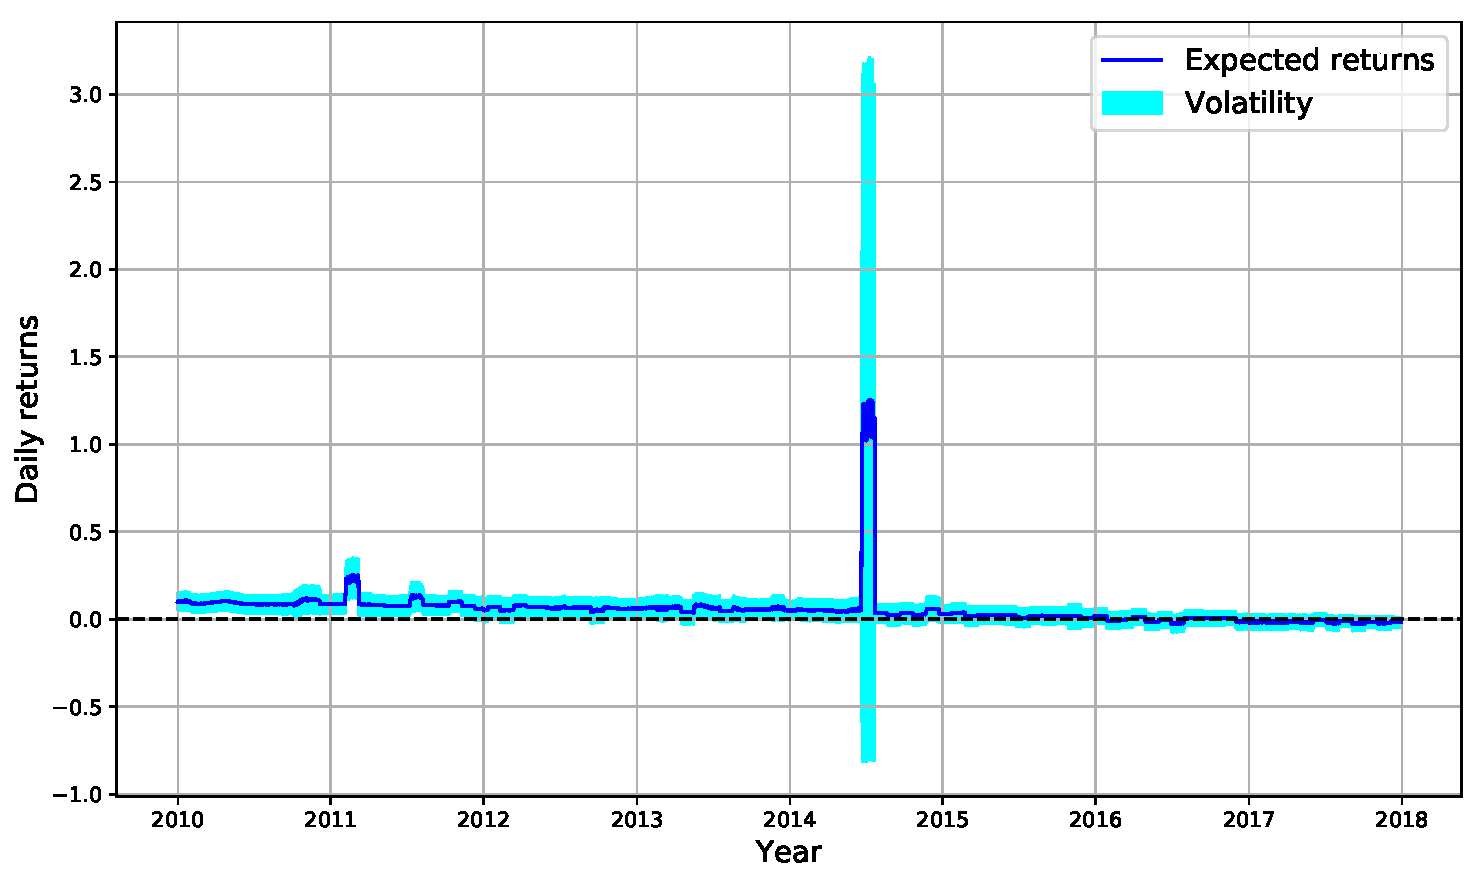
\includegraphics[width=0.75\linewidth]{figures/exp_ret_yearly.pdf}
\caption{Predicted returns for Case I}
\label{fig:ret_yrly}
\end{figure}  

In figure \ref{fig:ret_yrly}, we can observe that the predicted returns are strictly positive from 2010 to 2016. This can be due to the continuous increment of prices in the market. Although, the trend of the returns is decreasing except for peaks in 2011 and 2014. 


\subsection{Case II}
In this case, the performances computed at a shift of 22 days with the back-test window length of 10 years are used. The in-sample window of 10 years (starting from 2000-2009) with the step of 22 days is used for calibration and the returns are predicted from 2010 to 2017 sequentially. The predicted returns calculated for period from 2010-01-01 to 2017-12-31 are shown in figure \ref{fig:ret_mnthly10}.

\begin{figure}[h!] 
\centering
 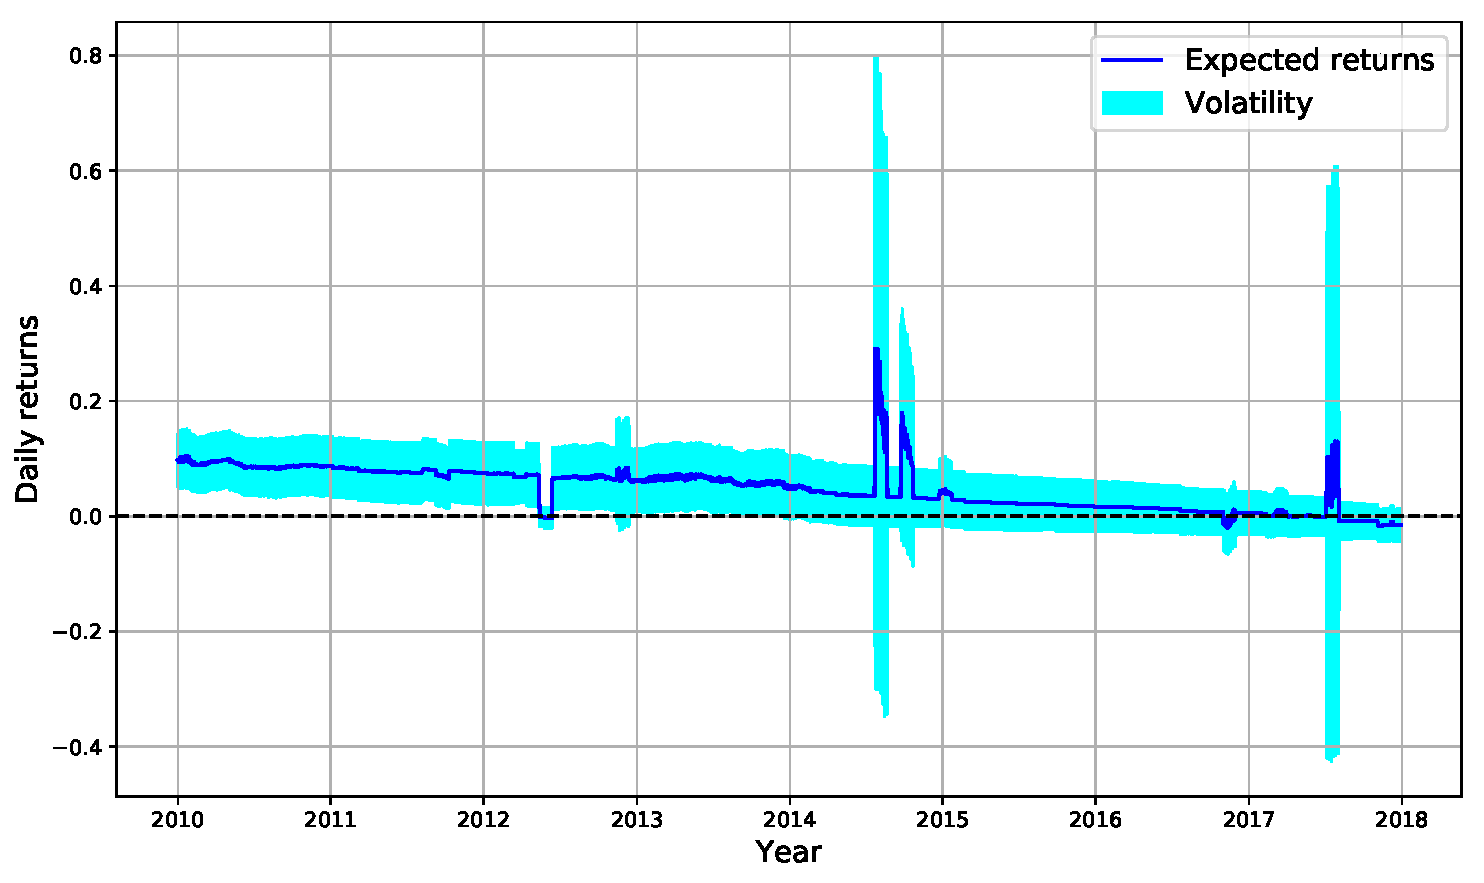
\includegraphics[width=0.75\linewidth]{figures/exp_ret_llf10.pdf}
\caption{Predicted returns for Case II}
\label{fig:ret_mnthly10}
\end{figure}  


In figure \ref{fig:ret_mnthly10}, we can observe that the predicted returns are mostly positive from 2010 to 2016 and follow a decreasing trend. The same behavior is observed for returns for in figure \ref{fig:ret_yrly}. Apart from the similarities, a drawdown in returns can be seen for 2012.



\subsection{Case III}
In this case, the performances computed at a shift of 22 days with the back-test window length of 10 years are used. The in-sample window of 5 years (starting from 2000-2004) with the step of 22 days is used for calibration and the returns are predicted from 2005 to 2017 sequentially. The predicted returns calculated for period from 2005-01-01 to 2017-12-31 are shown in figure \ref{fig:ret_mnthly5}.

\begin{figure}[h!] 
\centering
 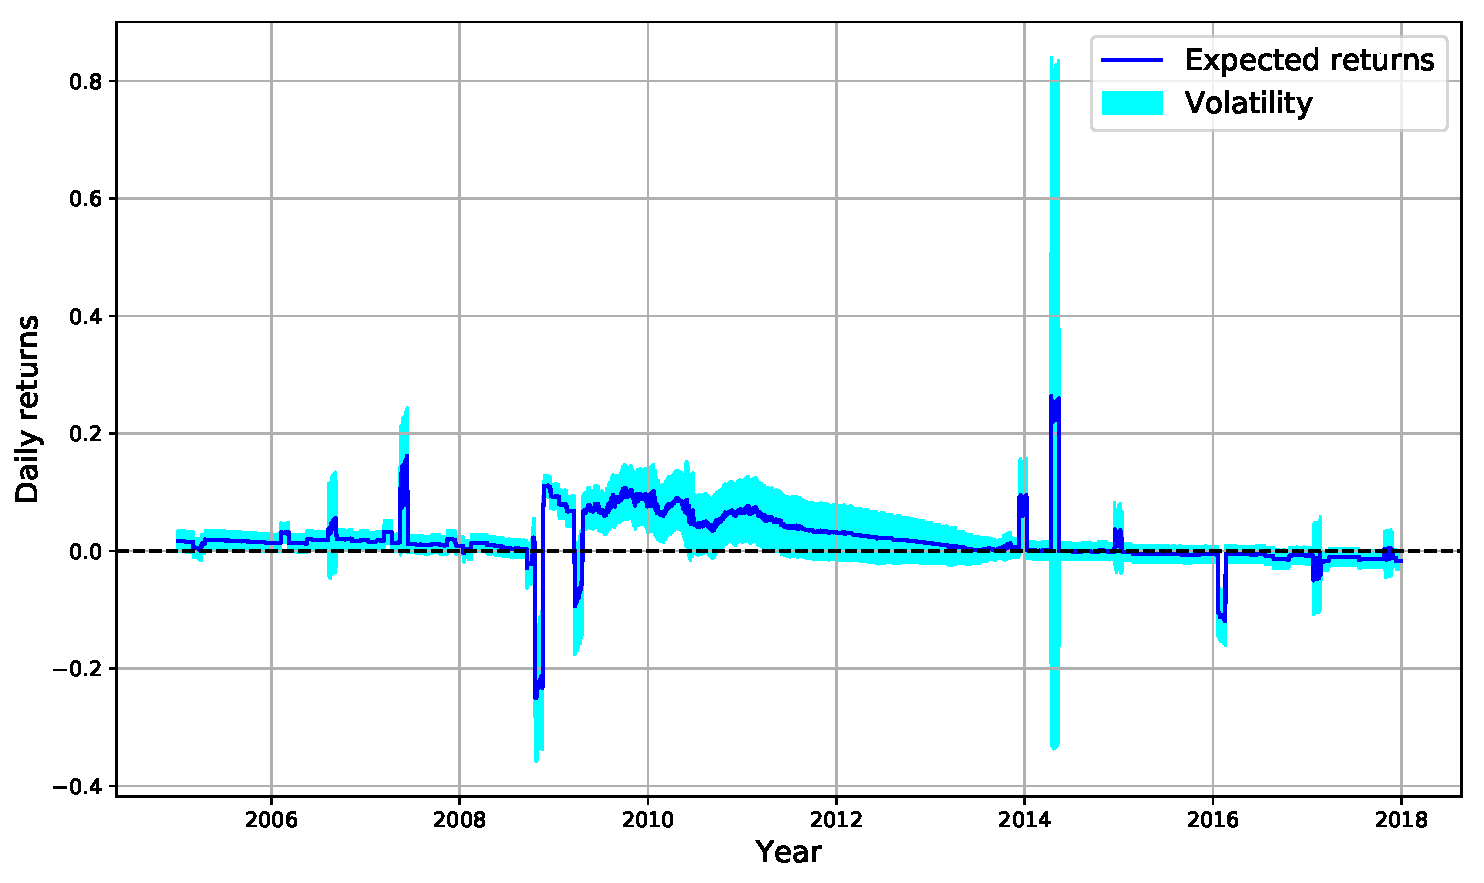
\includegraphics[width=0.75\linewidth]{figures/exp_ret_llf5.pdf}
\caption{Predicted returns for Case III}
\label{fig:ret_mnthly5}
\end{figure}  


In figure \ref{fig:ret_mnthly5}, we can observe that the predicted returns closely follow the actual return of the index, and is mostly positive from 2005-2015. We also observe negative returns for period 2008-2009 which seems to be relevant due to the occurrence of the financial crisis in 2008-2009.


\section{Statistical analysis results}
As explained in section 4.1, the next step is to generate a trading signal from predicted returns and volatilities using various trading strategies. We generated signal using two different trading strategies. The first strategy to generate the trading signal ($s(t)$) is given below:
\begin{equation*} \label{eqn:signal}
s(t) = 
\begin{cases}
  Buy\ (+1), & \text{if} \quad r(t) > 0.01 \\
  Short\ (-1), & \text{if} \quad r(t) < -0.01 \\
  Idle\ (0),  & \text{else}
\end{cases}
\end{equation*}

The other strategy used is as follow:
\begin{equation*} \label{eqn:signal}
s(t) = 
\begin{cases}
  Buy\ (+1), & \text{if} \quad r(t) > 1*\sigma(t) \\
  Short\ (-1), & \text{if} \quad r(t) < -1*\sigma(t) \\
  Idle\ (0),  & \text{else}
\end{cases}
\end{equation*}


We use these strategies to generate a trading signal for predicted returns obtained for all 3 cases. The trading signals and corresponding trading returns calculated using equation \ref{eqn:ret} for first strategy are shown in figure \ref{fig:t1}, \ref{fig:t2} and \ref{fig:t3}.

\begin{figure}[h!] 
\begin{tabular}{cc}
\centering 
 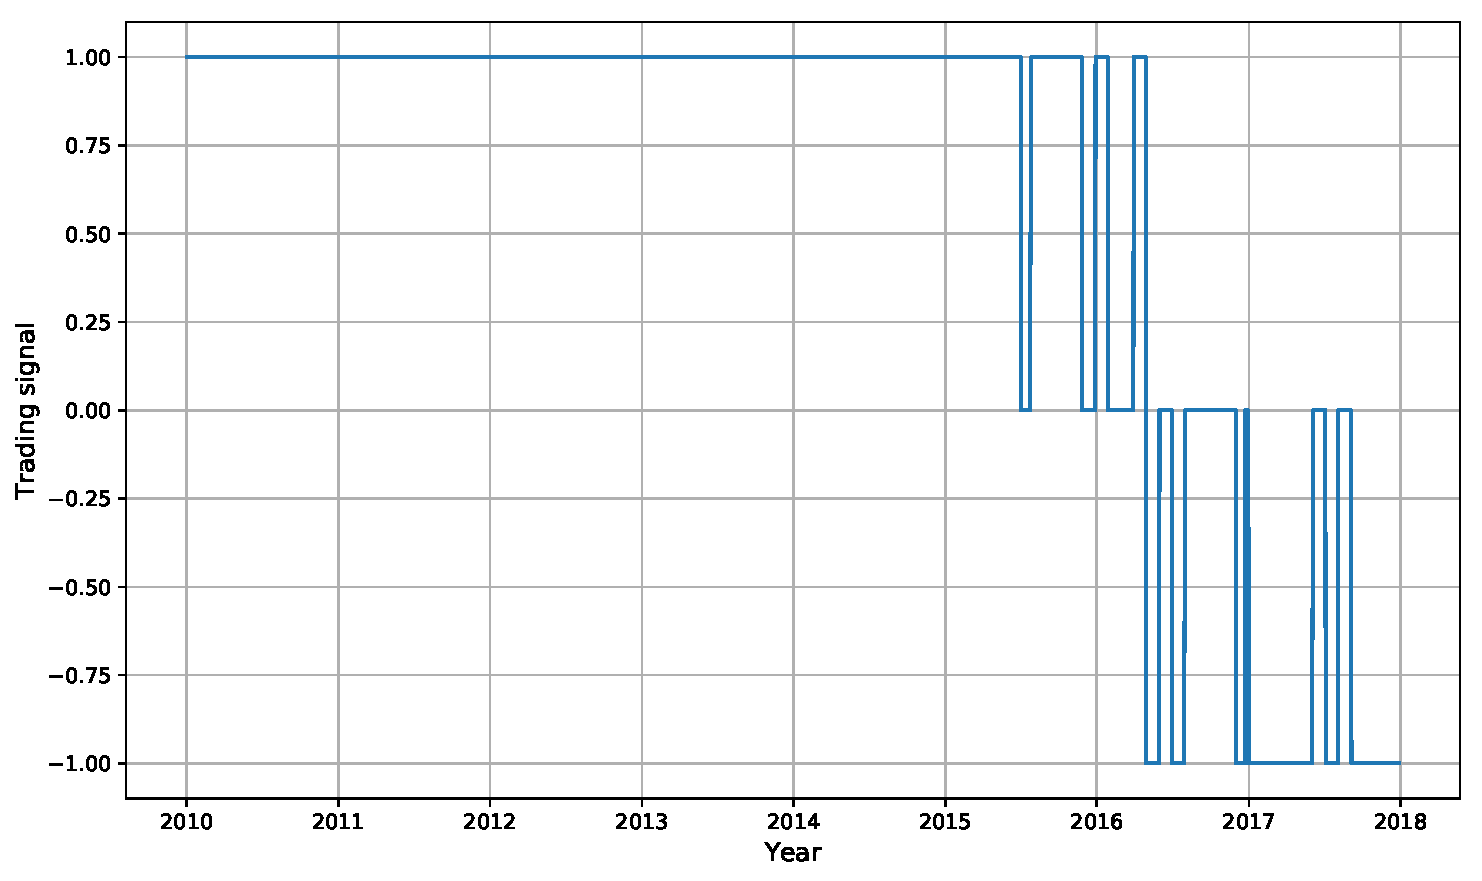
\includegraphics[width=0.5\linewidth]{figures/tradingSig_yearly_llf10.pdf} & 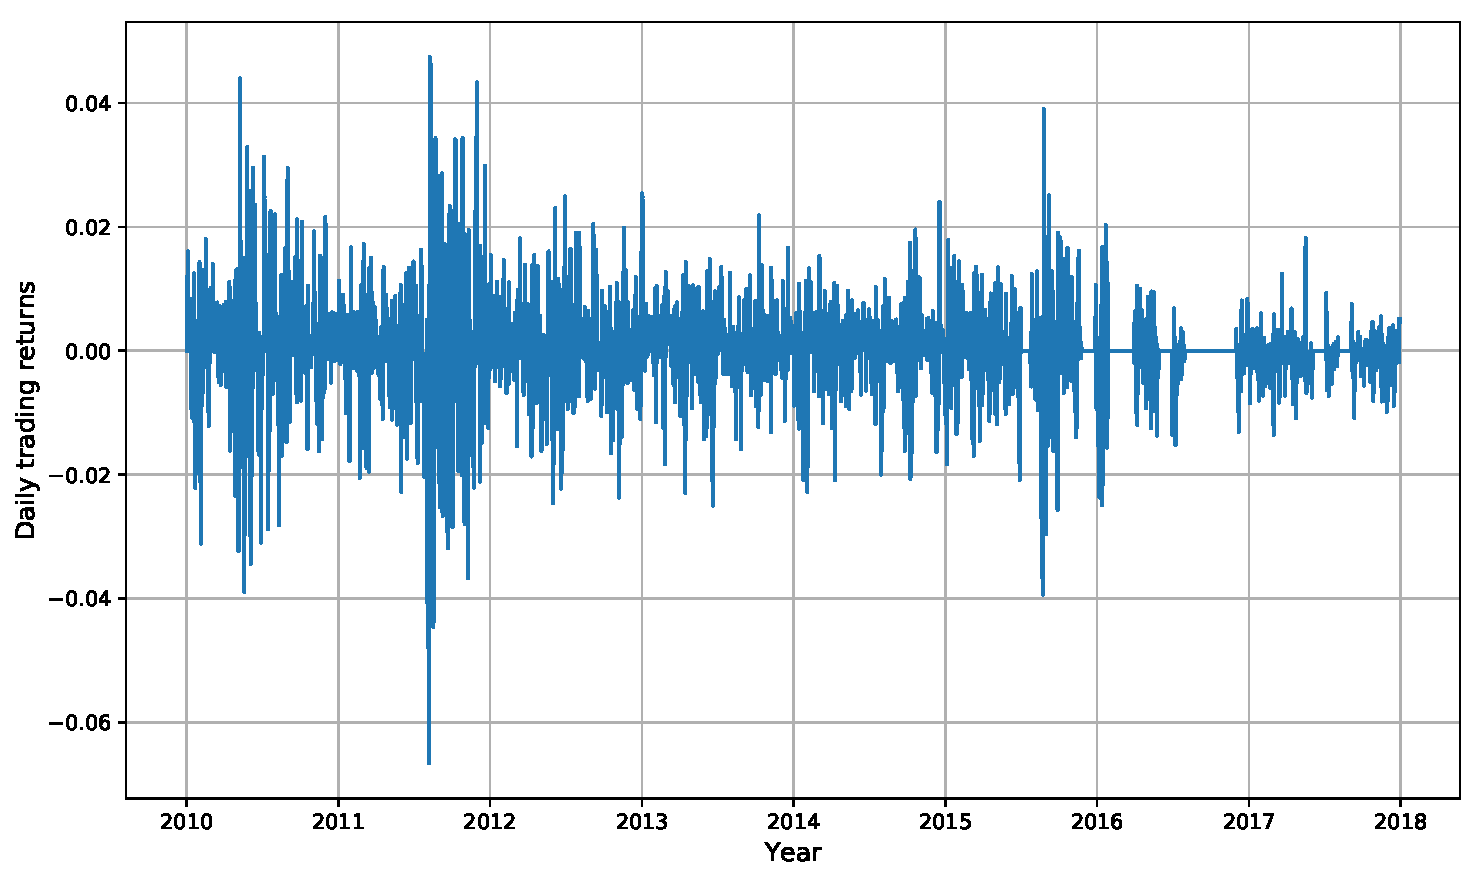
\includegraphics[width=0.5\linewidth]{figures/tradingRet_yearly_llf10.pdf} \\
  (a) & (b)
\end{tabular}
\caption{Results for Case I : (a) trading signal, (b) trading returns}
\label{fig:t1}
\end{figure}



\begin{figure}[h!] 
\begin{tabular}{cc}
\centering 
 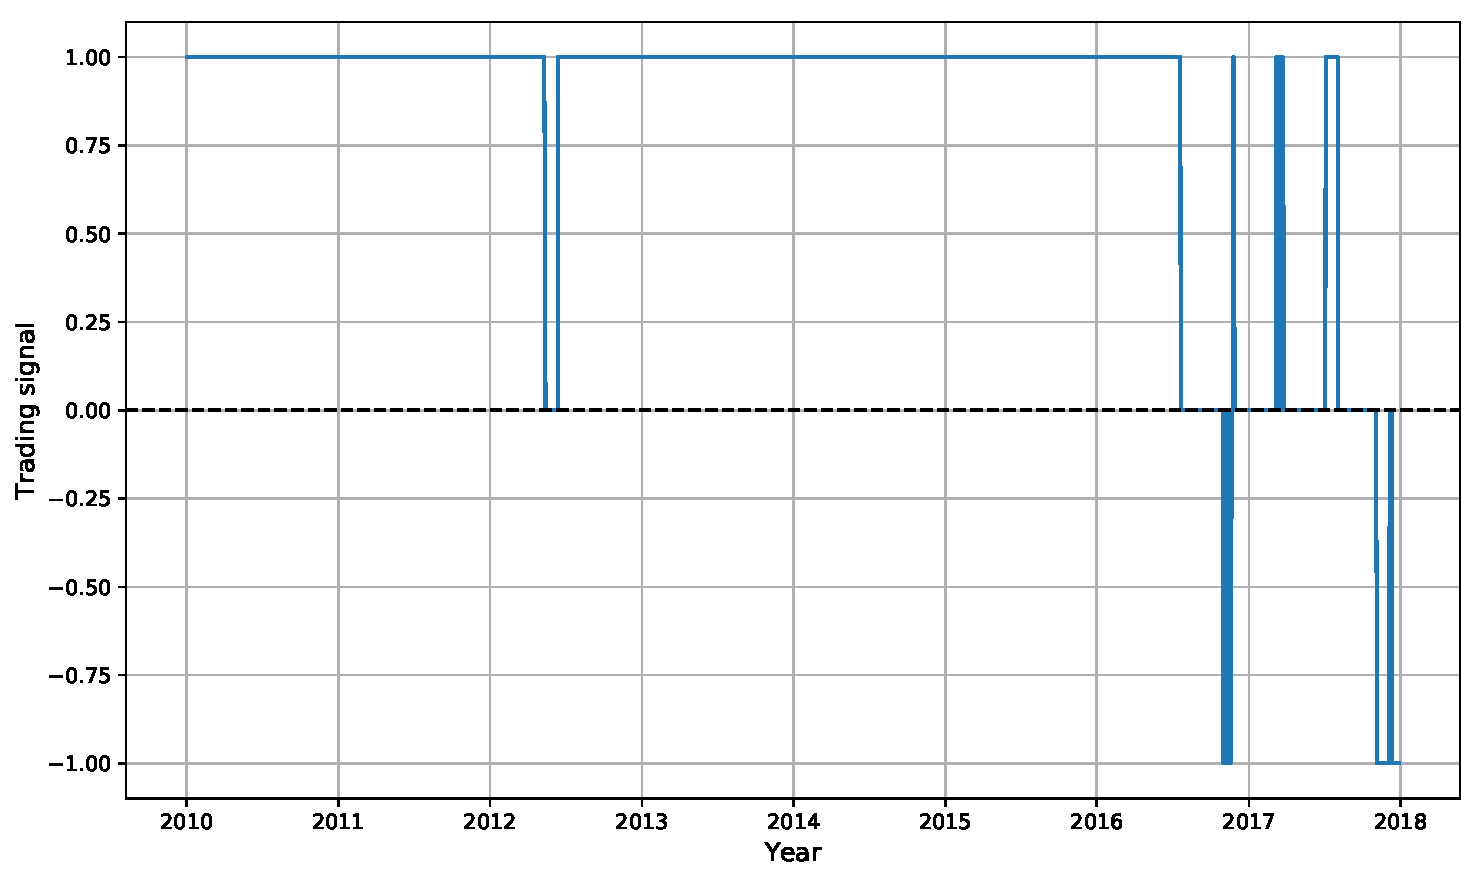
\includegraphics[width=0.5\linewidth]{figures/tradingSig_llf10.pdf} & 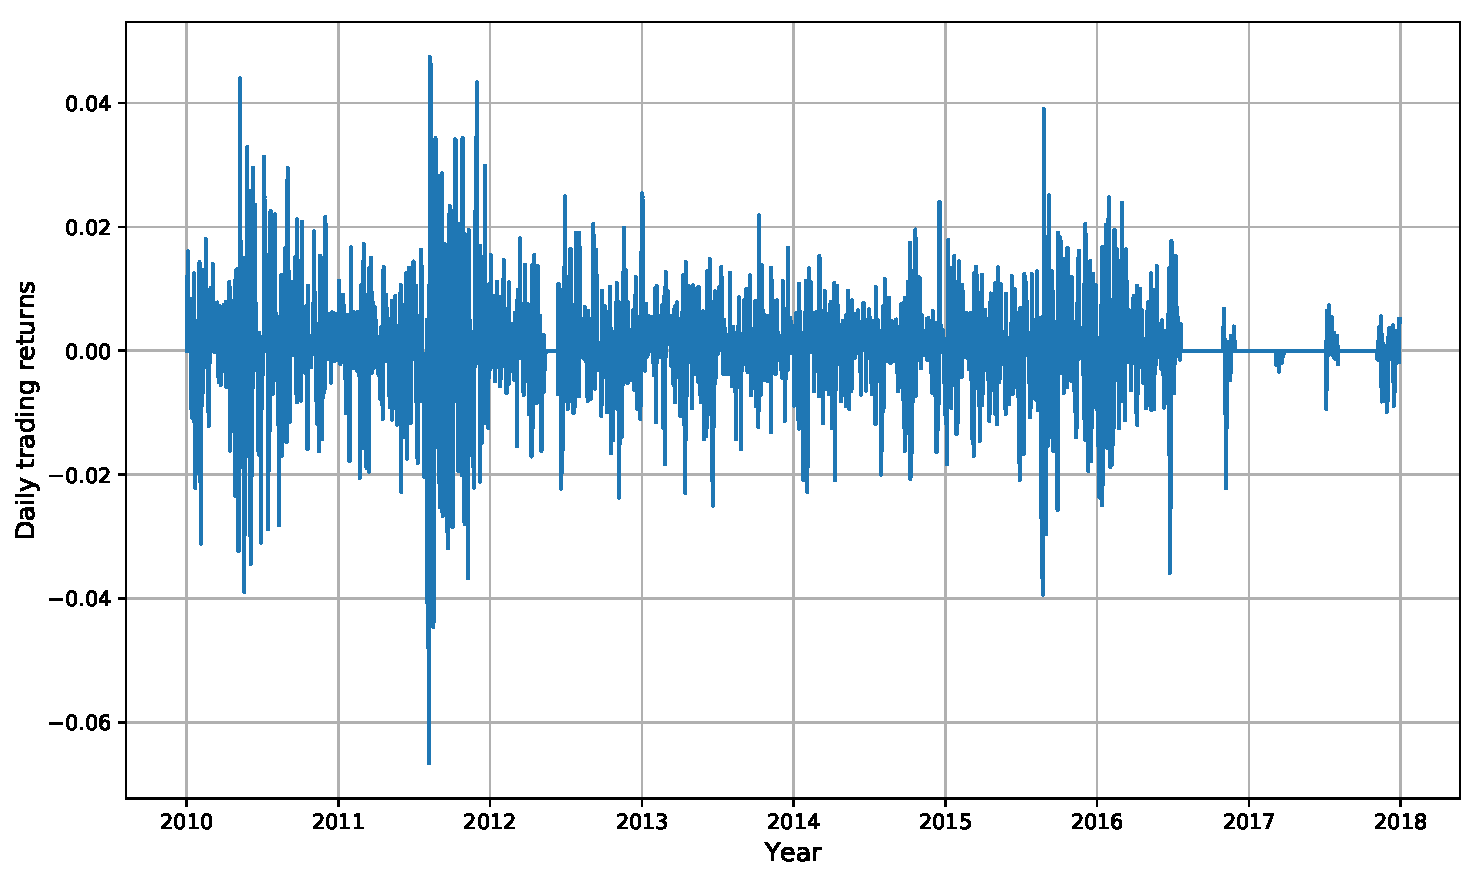
\includegraphics[width=0.5\linewidth]{figures/tradingRet_llf10.pdf} \\
  (a) & (b)
\end{tabular}
\caption{Results for Case II : (a) trading signal, (b) trading returns}
\label{fig:t2}
\end{figure}

\begin{figure}[h!] 
\begin{tabular}{cc}
\centering 
 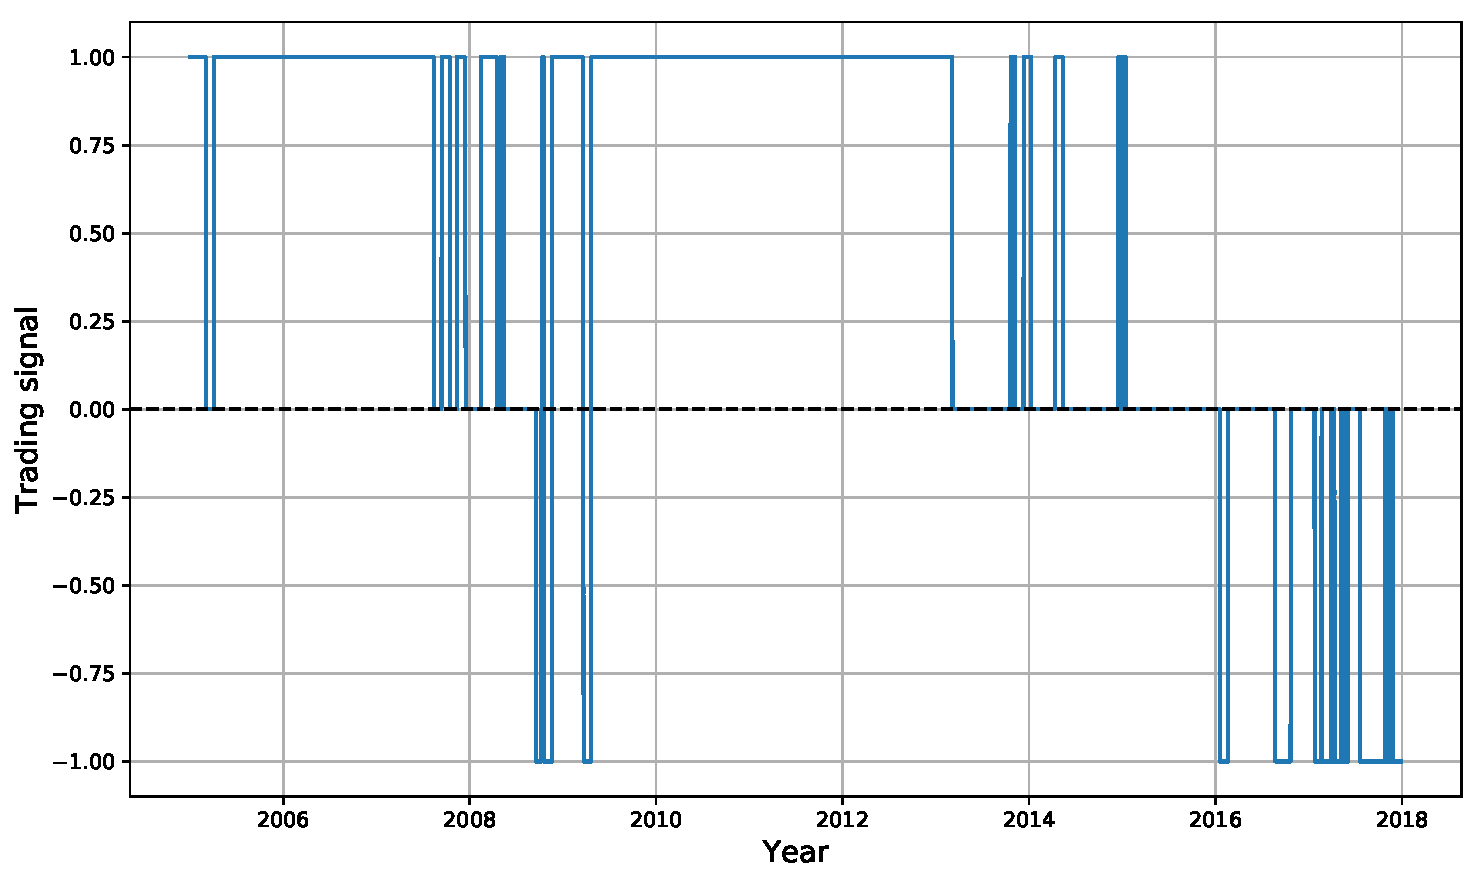
\includegraphics[width=0.5\linewidth]{figures/tradingSig_llf5.pdf} & 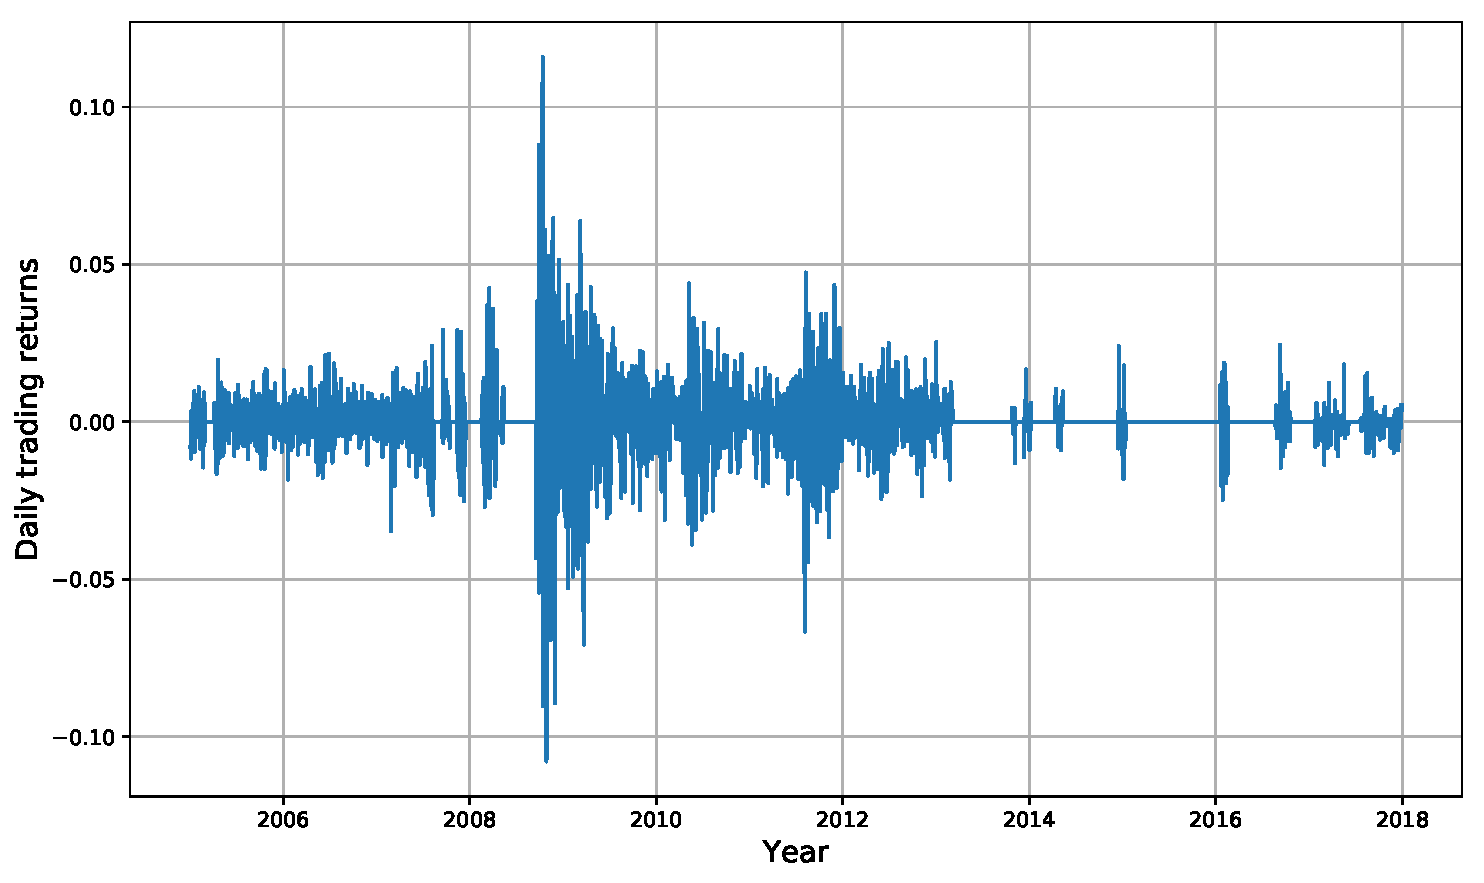
\includegraphics[width=0.5\linewidth]{figures/tradingRet_llf5.pdf} \\
\end{tabular}
\caption{Results for Case III : (a) trading signal, (b) trading returns}
\label{fig:t3}
\end{figure}

\subsection{Comparison with Random strategies}

The model can now be evaluated by comparing SABM trading returns obtained from first trading strategy against returns from randomly generated strategies, as explained in section \ref{ssec:random}. We generated 10,000 random strategies with the constraint of the same number of buy and short days for all the 3 cases. 
The performance of SABM for first strategy in terms of daily Profit and Loss (P\&L) for all the three cases are shown in figure \ref{fig:pnl1}, \ref{fig:pnl2} and \ref{fig:pnl3}. 

\begin{figure}[h!]
\centering 
 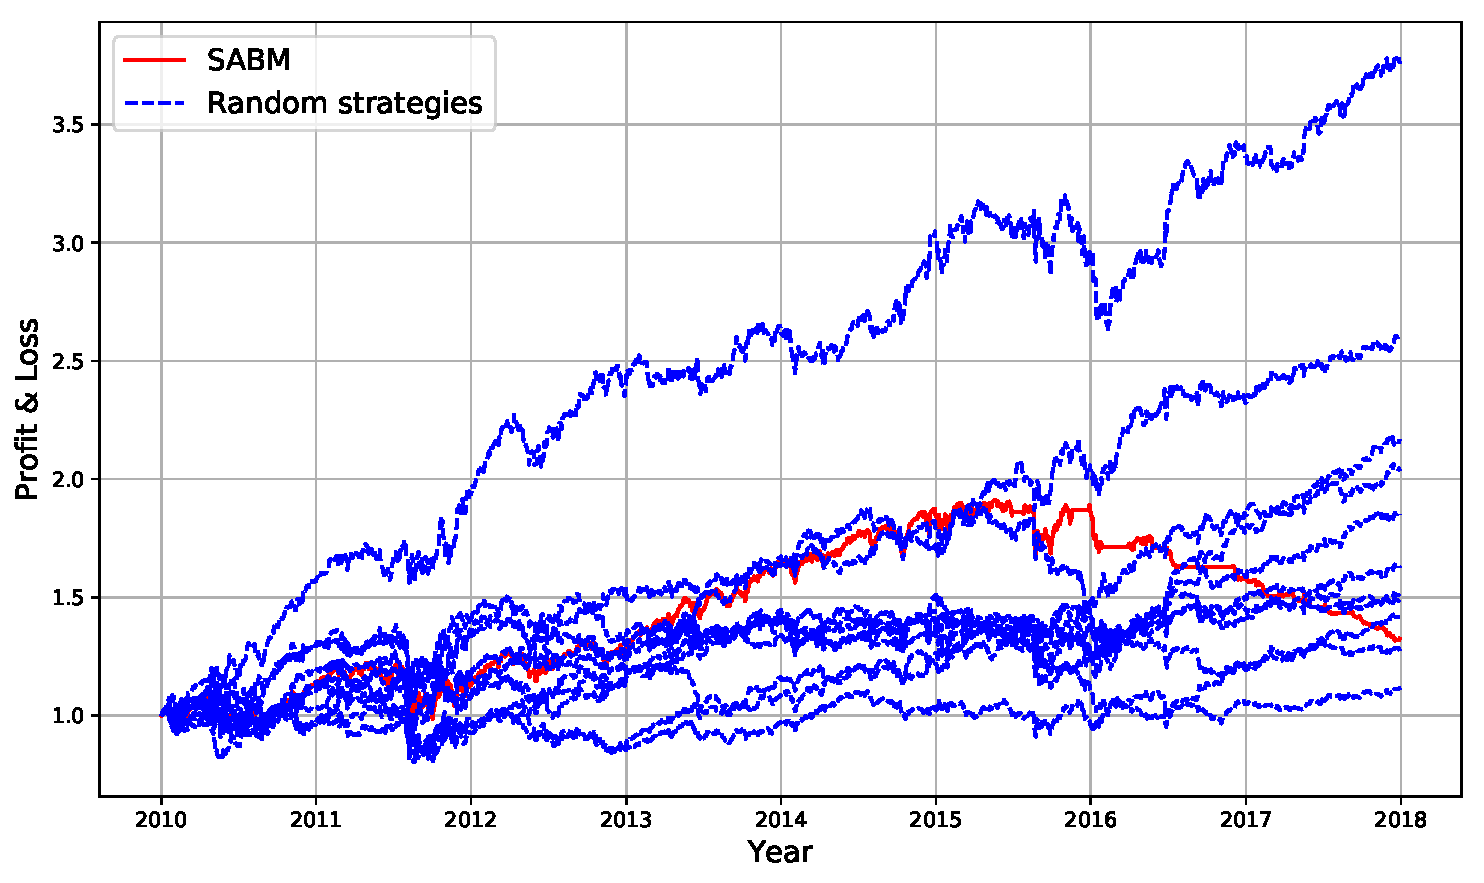
\includegraphics[width=0.75\linewidth]{figures/pnls_yearly.pdf} 
\caption{Daily Profit and Loss for Case I: SABM in red, Random strategies in blue}
\label{fig:pnl1}
\end{figure}

\begin{figure}[h!] 
\centering 
 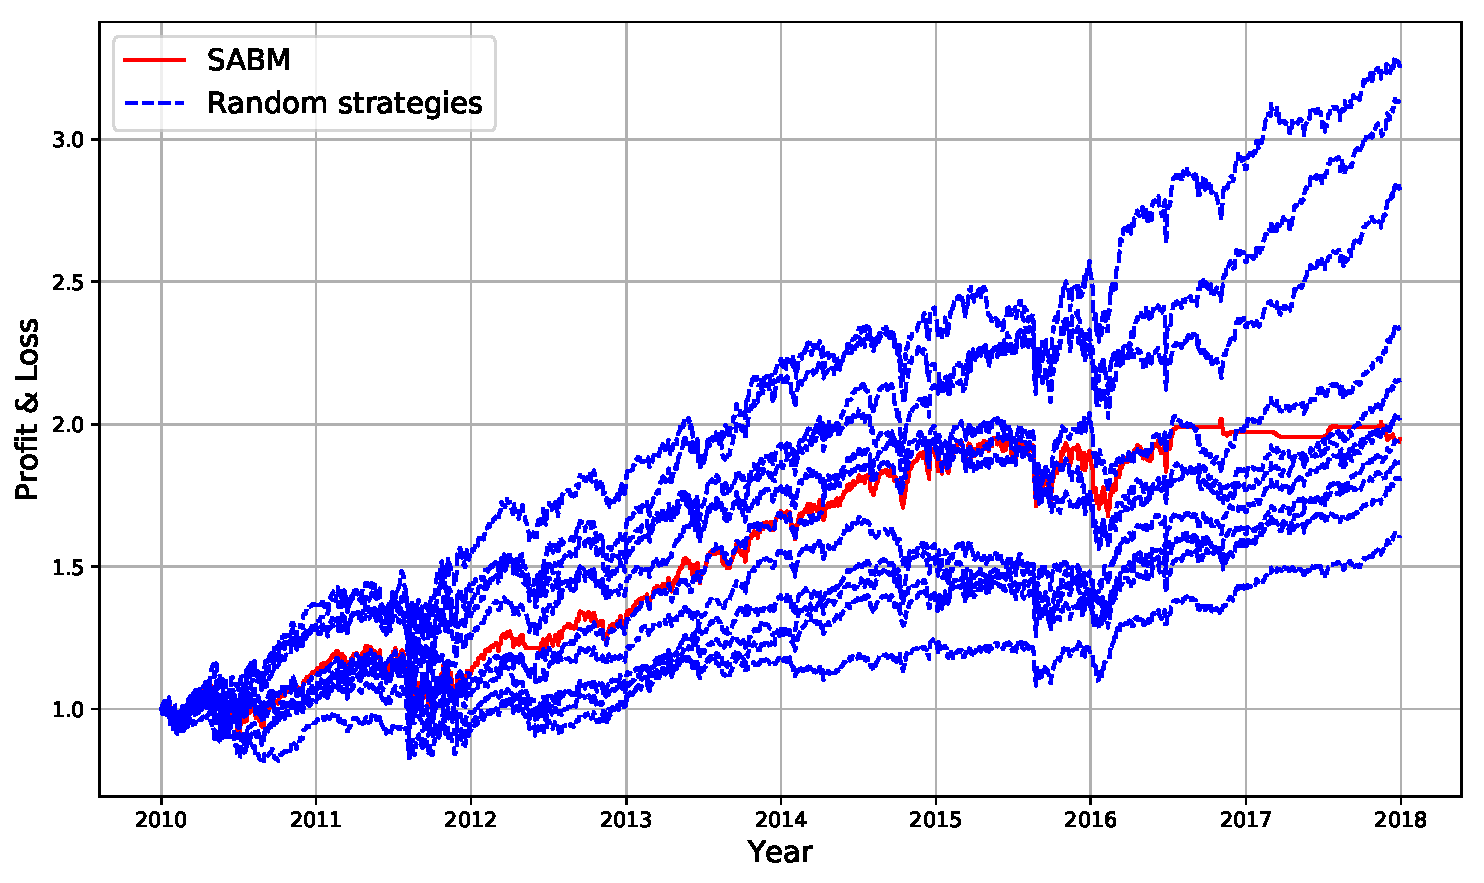
\includegraphics[width=0.75\linewidth]{figures/pnls_llf10.pdf} 
\caption{Daily Profit and Loss for Case II: SABM in red, Random strategies in blue}
\label{fig:pnl2}
\end{figure}

\begin{figure}[h!] 
\centering 
 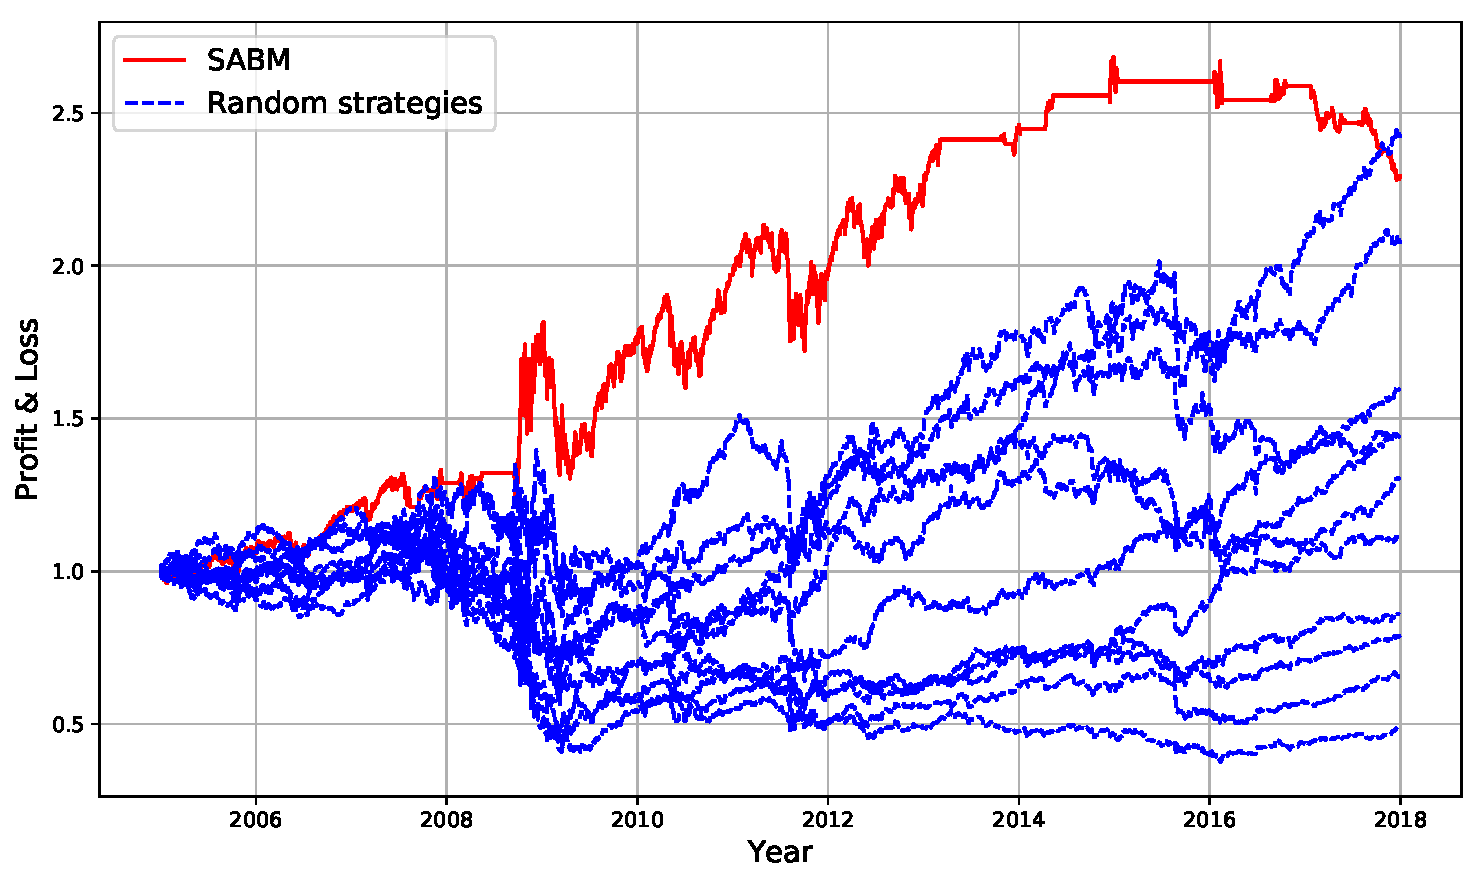
\includegraphics[width=0.75\linewidth]{figures/pnls_llf5.pdf} 
\caption{Daily Profit and Loss for Case III: SABM in red, Random strategies in blue}
\label{fig:pnl3}
\end{figure}

In the P\&L graphs for all 3 cases, the P\&L for Case III is better than the other two cases. In order to validate, we calculate the value of three performance indicators explained in \ref{ssec:random}. These indicators are shown in the table \ref{table:random}. 

\begin{table}[h!]
\begin{center}
\begin{tabular}{|c|cc|cc|cc|}
\hline
    \multicolumn{1}{|c|}{}&  \multicolumn{2}{|c|}{Sharpe ratio} & \multicolumn{2}{|c|}{Maximum drawdown} & \multicolumn{2}{|c|}{CAGR}\\
% \hline
    &  SABM &  Better than(\%) & SABM & Better than(\%) & SABM & Better than(\%) \\
\hline
    Case I &  0.451 &   21.42 &   0.31  &    21.33  & 0.041  & 21.77 \\
    Case II &  0.24 &   37.73 &   0.64  &    64.21  & 0.1    & 44.47  \\
    Case III &  0.393 &   83.3 &   0.457 &    91.8  & 0.072  & 86.31 \\
\hline
\end{tabular}
\end{center}
\caption{Results for different performance indicators}
\label{table:random}
\end{table}

The table \ref{table:random} shows the performance of our model in terms of Sharpe ratio, maximum drawdown, and CAGR for all 3 cases. The performance of our strategy is compared with the performance of random strategies. In case of Sharpe ratio and CAGR, we count the number of random strategies for which the value is less than the value of SABM. This number is shown as a percentage of total strategies in column ``Better than (\%)''. Similarly, for maximum drawdown, the number of random strategies for which the drawdown is more than the drawdown of our SABM, is calculated. We can observe the improvement in percentage for all three indicators for Case III. 


\section{Linear regression}
The other method to evaluate our model is to run linear regression using with \textit{FAMA-FRENCH 3 factors model}, as explained in section \ref{ssec:linear}.
We used the trading returns calculated as a dependent variable. The regression was run for all 3 cases. The regression was run using \textit{ols} functionality from \textit{statsmodels} python package. The results for Case I, II and III are shown in figure \ref{table:lr_case1}, \ref{table:lr_case2} and \ref{table:lr_case3} respectively.


\begin{table}
\center
\begin{tabular}{|lc|lc|}
\hline
\textbf{Dep. Variable:}    &     exp\_ret      & \textbf{  R-squared:         } &     0.114   \\
\textbf{Model:}            &       OLS        & \textbf{  Adj. R-squared:    } &     0.113   \\
\textbf{Method:}           &  Least Squares   & \textbf{  F-statistic:       } &     128.7   \\
\textbf{Log-Likelihood:    } &    6775.5 & \textbf{  Prob (F-statistic):} &  2.47e-53   \\
\textbf{No. Observations:} &        2013      & \textbf{  AIC:               } & -1.355e+04  \\
\textbf{Df Residuals:}     &        2010      & \textbf{  BIC:               } & -1.353e+04  \\
\textbf{Df Model:}         &           2      & \textbf{                     } &             \\
\hline
\end{tabular}

\bigskip

\begin{tabular}{|l|cccccc|}
\hline

                   & \textbf{coef} & \textbf{std err} & \textbf{t} & \textbf{P$>$$|$t$|$} & \textbf{[0.025} & \textbf{0.975]}  \\
\hline
\textbf{Intercept} &       0.0002  &        0.000     &     0.947  &         0.344        &       -0.000    &        0.001     \\
\textbf{SMB}       &       0.0046  &        0.000     &    12.882  &         0.000        &        0.004    &        0.005     \\
\textbf{HML}       &       0.0039  &        0.000     &    10.062  &         0.000        &        0.003    &        0.005     \\
\hline
\end{tabular}

\bigskip

\begin{tabular}{|lc|lc|}
\hline

\textbf{Omnibus:}       & 224.686 & \textbf{  Durbin-Watson:     } &    2.035  \\
\textbf{Prob(Omnibus):} &   0.000 & \textbf{  Jarque-Bera (JB):  } & 1629.264  \\
\textbf{Skew:}          &  -0.242 & \textbf{  Prob(JB):          } &     0.00  \\
\textbf{Kurtosis:}      &   7.381 & \textbf{  Cond. No.          } &     2.09  \\
\hline
\end{tabular}
\caption{Regression Results for Case I}
\label{table:lr_case1}
\end{table}



The table \ref{table:lr_case1} shows the value of alpha (excess return) to be 0.01\%, which is positive. Also, the coefficients of the two factors, SMB and HML, are positive and statistically significant at 10\% level. The value of $R^2$ is 14\

\begin{table}
\centering
\begin{tabular}{|lc|lc|}
\hline
\textbf{Dep. Variable:}    &     exp\_ret      & \textbf{  R-squared:         } &     0.137   \\
\textbf{Model:}            &       OLS        & \textbf{  Adj. R-squared:    } &     0.136   \\
\textbf{Method:}           &  Least Squares   & \textbf{  F-statistic:       } &     159.1   \\
\textbf{Log-Likelihood:} &    6768.9 & \textbf{  Prob (F-statistic):} &  7.34e-65   \\
\textbf{No. Observations:} &        2013      & \textbf{  AIC:               } & -1.353e+04  \\
\textbf{Df Residuals:}     &        2010      & \textbf{  BIC:               } & -1.351e+04  \\
\textbf{Df Model:}         &           2      & \textbf{                     } &             \\
\hline
\end{tabular}

\bigskip

\begin{tabular}{|l|cccccc|}
\hline

                   & \textbf{coef} & \textbf{std err} & \textbf{t} & \textbf{P$>$$|$t$|$} & \textbf{[0.025} & \textbf{0.975]}  \\
\hline
\textbf{Intercept} &       0.0004  &        0.000     &     1.975  &         0.048        &     2.55e-06    &        0.001     \\
\textbf{SMB}       &       0.0051  &        0.000     &    14.116  &         0.000        &        0.004    &        0.006     \\
\textbf{HML}       &       0.0045  &        0.000     &    11.446  &         0.000        &        0.004    &        0.005     \\
\hline
\end{tabular}

\bigskip

\begin{tabular}{|lc|lc|}
\hline
\textbf{Omnibus:}       & 226.654 & \textbf{  Durbin-Watson:     } &    2.020  \\
\textbf{Prob(Omnibus):} &   0.000 & \textbf{  Jarque-Bera (JB):  } & 1579.960  \\
\textbf{Skew:}          &  -0.271 & \textbf{  Prob(JB):          } &     0.00  \\
\textbf{Kurtosis:}      &   7.306 & \textbf{  Cond. No.          } &     2.09  \\
\hline
\end{tabular}
\caption{Regression Results for Case II}
\label{table:lr_case2}
\end{table}

 
The table \ref{table:lr_case2} shows the value of alpha to be 0.02\%, which is also positive. Also, the coefficients of the two factors, SMB and HML, are positive and statistically significant at 10\% level. The value of $R^2$ is 16.7\%.


\begin{table}
\centering
\begin{tabular}{|lc|lc|}
\hline
\textbf{Dep. Variable:}    &     exp\_ret      & \textbf{  R-squared:         } &     0.074   \\
\textbf{Model:}            &       OLS        & \textbf{  Adj. R-squared:    } &     0.074   \\
\textbf{Method:}           &  Least Squares   & \textbf{  F-statistic:       } &     131.1   \\
\textbf{Log-Likelihood:} &    10373. & \textbf{  Prob (F-statistic):} &  1.64e-55   \\
\textbf{No. Observations:} &        3272      & \textbf{  AIC:               } & -2.074e+04  \\
\textbf{Df Residuals:}     &        3269      & \textbf{  BIC:               } & -2.072e+04  \\
\textbf{Df Model:}         &           2      & \textbf{                     } &             \\
\hline
\end{tabular}

\bigskip

\begin{tabular}{|l|cccccc|}
\hline
                   & \textbf{coef} & \textbf{std err} & \textbf{t} & \textbf{P$>$$|$t$|$} & \textbf{[0.025} & \textbf{0.975]}  \\
\hline
\textbf{Intercept} &       0.0003  &        0.000     &     1.647  &         0.100        &    -5.57e-05    &        0.001     \\
\textbf{SMB}       &       0.0042  &        0.000     &    13.358  &         0.000        &        0.004    &        0.005     \\
\textbf{HML}       &       0.0028  &        0.000     &    10.217  &         0.000        &        0.002    &        0.003     \\
\hline
\end{tabular}

\bigskip

\begin{tabular}{|lc|lc|}
\textbf{Omnibus:}       & 903.068 & \textbf{  Durbin-Watson:     } &     2.167  \\
\textbf{Prob(Omnibus):} &   0.000 & \textbf{  Jarque-Bera (JB):  } & 78120.161  \\
\textbf{Skew:}          &   0.243 & \textbf{  Prob(JB):          } &      0.00  \\
\textbf{Kurtosis:}      &  26.933 & \textbf{  Cond. No.          } &      1.78  \\
\hline
\end{tabular}
\caption{Regression Results for Case III}
\label{table:lr_case3}
\end{table}

The table \ref{table:lr_case3} shows the value of alpha (excess return) to be 0.01\%, which is also positive. Also, the coefficients of the two factors, SMB and HML, are positive and statistically significant at 5\% level. The value of $R^2$ is 0.36\%, which is significantly low.